\documentclass[12pt,a4paper]{article}

\usepackage[top=1in,bottom=1in,left=1.15in,right=1.15in]{geometry}
\usepackage{graphicx}
\usepackage{amsmath}
\usepackage{booktabs}
\usepackage{array}
\usepackage{hyperref}
\usepackage{setspace}
\usepackage{parskip}
\usepackage[round]{natbib}
\usepackage{float}
\usepackage{caption}
\usepackage{xcolor}
\usepackage{fancyhdr}
\usepackage{titlesec}
\usepackage{mdframed}
\usepackage{enumitem}

\hypersetup{colorlinks=true,linkcolor=blue!60!black,
             citecolor=blue!60!black,urlcolor=blue!70!black}
\onehalfspacing
\setlength{\parindent}{0pt}
\setlength{\parskip}{8pt}

\titleformat{\section}{\large\bfseries\color{blue!70!black}}{{\thesection.}}{0.5em}{}[\titlerule]
\titleformat{\subsection}{\normalsize\bfseries}{{\thesubsection}}{0.5em}{}

\pagestyle{fancy}
\fancyhf{}
\rhead{\small Song Popularity Score}
\lhead{\small Probability \& Statistics Project --- 2026}
\cfoot{\thepage}
\renewcommand{\headrulewidth}{0.4pt}

\newmdenv[backgroundcolor=blue!5,linecolor=blue!40,linewidth=0.8pt,
  innerleftmargin=10pt,innerrightmargin=10pt,
  innertopmargin=8pt,innerbottommargin=8pt]{infobox}

% Auto-generated by generate_report.py — DO NOT EDIT MANUALLY

\begin{document}

%% Title Page
\begin{titlepage}
  \centering\vspace*{1.5cm}
  {\Large\bfseries University Name Here\par}\vspace{0.3cm}
  {\large Department of Economics / Statistics\par}\vspace{2cm}
  \rule{\linewidth}{1.5pt}\\[0.4cm]
  {\LARGE\bfseries Determinants of Song Popularity Score on Spotify\\[0.3cm]
    A Regression and Machine Learning Analysis\par}
  \rule{\linewidth}{1.5pt}\vspace{1.5cm}
  {\large\bfseries Probability \& Statistics --- Group Project\par}\vspace{1cm}
  \begin{tabular}{ll}
    \textbf{Group Member 1:} & Name, Roll No. \\[4pt]
    \textbf{Group Member 2:} & Name, Roll No. \\[4pt]
    \textbf{Group Member 3:} & Name, Roll No. \\
  \end{tabular}\vspace{1.5cm}
  {\large\textbf{Instructor:} Prof.\ [Name Here]\par}\vspace{0.5cm}
  {\large\textbf{Submission:} May 5, 2026\par}\vfill
  {\small\textit{Analysis performed in Python 3.x using pandas, scikit-learn,
    statsmodels, matplotlib, seaborn, and scipy.}\\
    \textit{Report auto-generated dynamically from results.json}}
\end{titlepage}

\tableofcontents\newpage

%% 1. Introduction
\section{Introduction}
Spotify hosts over 100 million tracks and serves 600+ million monthly active
users. Each track carries a \textit{popularity score} (0--100) based on
recent play counts. This study identifies audio-feature determinants of that
score using a sample of $n = 500$ tracks.

\begin{infobox}
\textbf{Research Question:} To what extent do danceability, energy, loudness,
valence, tempo, and duration explain the Spotify Popularity Score?
\end{infobox}

We use two methods: \textbf{Multiple Linear Regression (MLR)} for
interpretability and \textbf{Random Forest (RF)} for predictive accuracy.
All code is written in \textbf{Python 3.x}.

%% 2. Literature Review
\section{Literature Review}
Pachet \& Roy (2011) argued that predicting hit songs purely from audio
features is difficult due to social and cultural factors. Interiano et al.\
(2018) found danceability and valence to be positively associated with chart
performance in 500,000+ Billboard entries. Ferreri et al.\ (2019) showed
Random Forest outperforms linear regression on Spotify data, with loudness
and energy as the top predictors. Park et al.\ (2022) demonstrated that
track duration has a negative effect on popularity in the streaming era.

\textbf{Hypotheses:}
\begin{itemize}[leftmargin=2em]
  \item[\textbf{H1:}] Danceability $\rightarrow$ positive effect.
  \item[\textbf{H2:}] Energy $\rightarrow$ positive effect.
  \item[\textbf{H3:}] Loudness $\rightarrow$ positive effect.
  \item[\textbf{H4:}] Valence $\rightarrow$ ambiguous effect.
  \item[\textbf{H5:}] Tempo $\rightarrow$ weak or ambiguous effect.
  \item[\textbf{H6:}] Duration $\rightarrow$ negative effect.
  \item[\textbf{H7:}] RF will produce lower MSE than MLR.
\end{itemize}

%% 3. Variables and Data
\section{Description of Variables and Data}

\subsection{Data Source}
Data: \textit{Spotify Tracks Dataset}, Kaggle (Pandya, 2023).\\
URL: \url{https://www.kaggle.com/datasets/maharshipandya/-spotify-tracks-dataset}\\
Original size: 114,000 tracks. Sample used: $n = 500$
(random\_state = 42). Train/test split: 400/100.

\subsection{Variable Definitions}
\begin{table}[H]
\centering\caption{Variable Definitions}
\begin{tabular}{>{\ttfamily}l l p{6cm} c}
\toprule
\textbf{Variable} & \textbf{Type} & \textbf{Definition} & \textbf{Sign} \\
\midrule
popularity    & Dependent   & Spotify score 0--100                 & ---  \\
danceability  & Independent & Suitability for dancing (0--1)        & $+$  \\
energy        & Independent & Intensity and activity (0--1)         & $+$  \\
loudness      & Independent & Overall loudness in dB                & $+$  \\
valence       & Independent & Musical positiveness (0--1)           & $\pm$\\
tempo         & Independent & Estimated BPM                         & $\pm$\\
duration\_min & Independent & Track length in minutes               & $-$  \\
\bottomrule
\end{tabular}
\end{table}

%% 4. Summary Statistics
\section{Summary Statistics}
\begin{table}[H]
\centering\caption{Descriptive Statistics ($n = 500$)}
\small
\begin{tabular}{lrrrrrrrrr}
\toprule
\textbf{Variable} & \textbf{Mean} & \textbf{Median} & \textbf{Mode} & \textbf{Std} & \textbf{Q1} & \textbf{Q3} & \textbf{Min} & \textbf{Max} & \textbf{Skew} \\
\midrule
  popularity      & 38.1960 & 40.0000 & 43.0000 & 19.6135 & 23.0000 & 52.0000 & 1.0000 & 88.0000 & +0.0508 \\
  danceability    & 0.5626 & 0.5825 & 0.6610 & 0.1719 & 0.4460 & 0.6880 & 0.0000 & 0.9160 & -0.4094 \\
  energy          & 0.6407 & 0.6895 & 0.6250 & 0.2542 & 0.4657 & 0.8562 & 0.0000 & 1.0000 & -0.5939 \\
  loudness        & -8.4088 & -7.3080 & -4.7190 & 4.8528 & -10.4250 & -5.1713 & -33.1390 & 0.2170 & -1.7833 \\
  valence         & 0.4693 & 0.4655 & 0.9620 & 0.2671 & 0.2455 & 0.6593 & 0.0000 & 0.9750 & +0.1902 \\
  tempo           & 122.9978 & 122.8995 & 90.0390 & 29.6558 & 99.9708 & 140.9585 & 0.0000 & 205.8640 & +0.1981 \\
  duration_min    & 3.8170 & 3.5892 & 2.0000 & 1.6830 & 2.9045 & 4.4043 & 0.5198 & 19.9010 & +3.2297 \\
\bottomrule
\multicolumn{10}{l}{\small Source: Kaggle; Python computation.}
\end{tabular}
\end{table}

\textbf{Discussion:} Popularity has a skewness of +0.0508, indicating a right-skewed distribution. Danceability mean = 0.5626; energy mean = 0.6407. Loudness ranges from -33.14 to 0.22 dB. Duration ranges from 0.52 to 19.90 minutes.

%% 5. Box Plots
\section{Box and Whisker Plots}
Variables normalised to $[0,1]$: $x_{\text{norm}} = (x - x_{\min}) / (x_{\max} - x_{\min})$. Outliers detected via $1.5\times$IQR rule.

\begin{figure}[H]
  \centering
  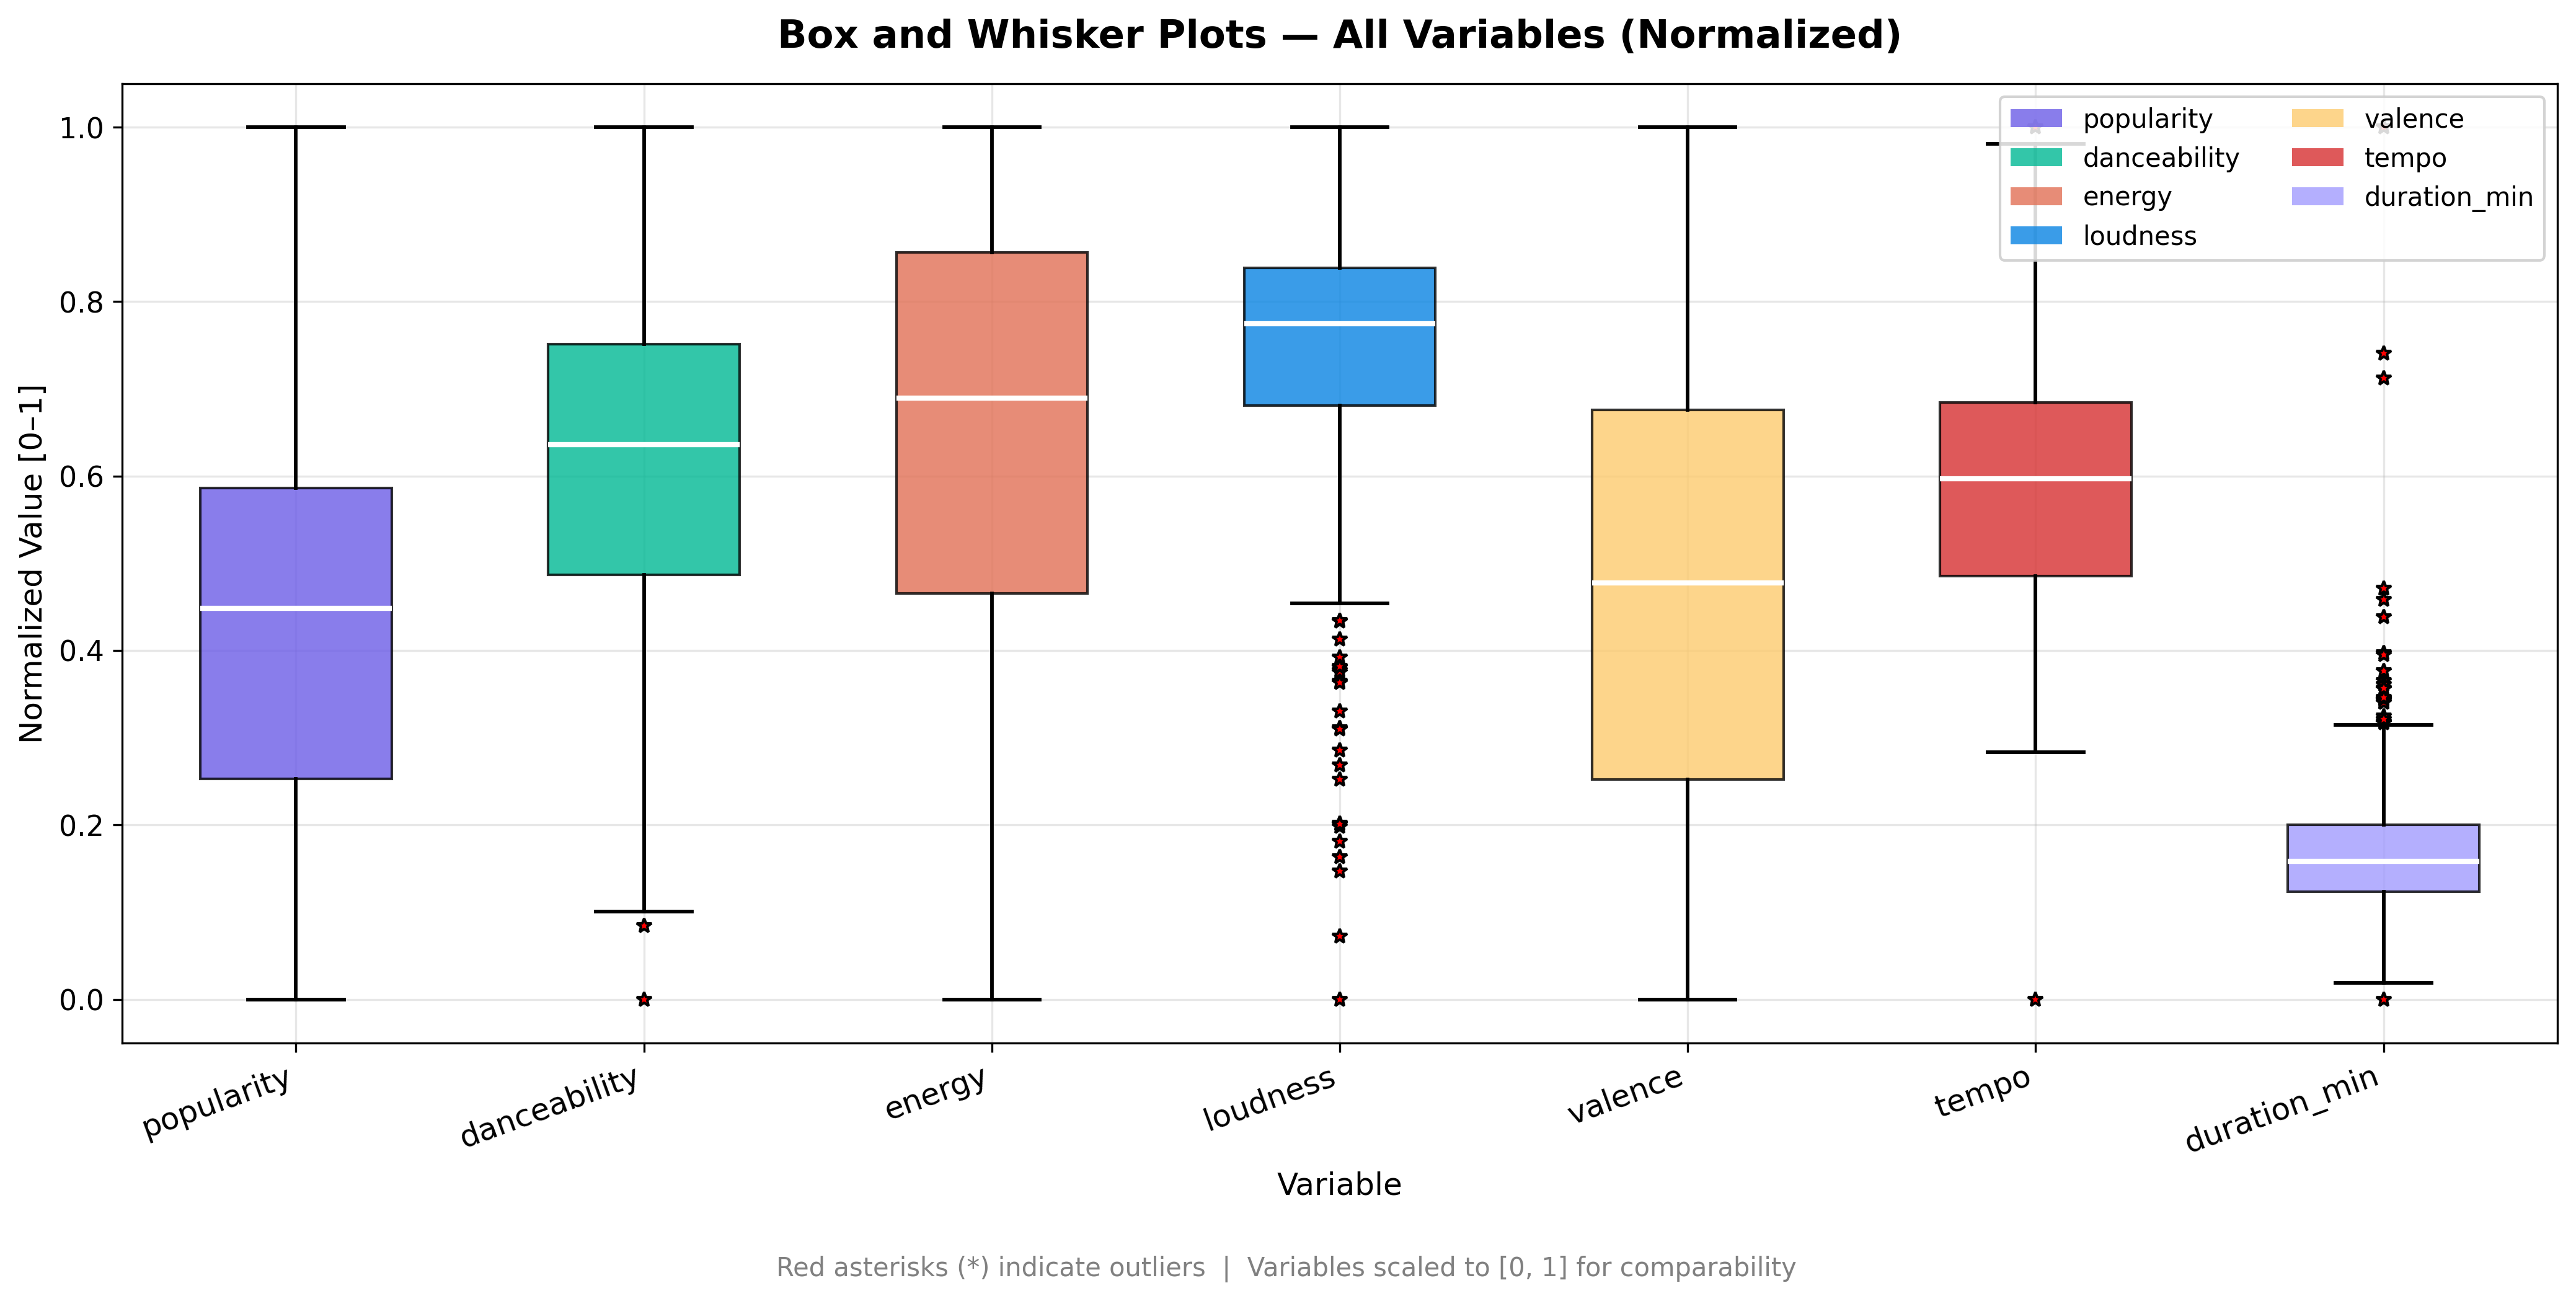
\includegraphics[width=\textwidth]{boxplot_all_variables.png}
  \caption{Box and Whisker Plots --- All Variables (Normalised, $n=500$). Red asterisks = outliers.}
\end{figure}

\textbf{Outlier counts (IQR rule):}
\begin{itemize}[leftmargin=2em]
  \item popularity: 0 outliers
  \item danceability: 2 outliers
  \item energy: 0 outliers
  \item loudness: 24 outliers
  \item valence: 0 outliers
  \item tempo: 2 outliers
  \item duration_min: 24 outliers
\end{itemize}

%% 6. Scatter Grid
\section{Scatter Plot Grid}
\begin{figure}[H]
  \centering
  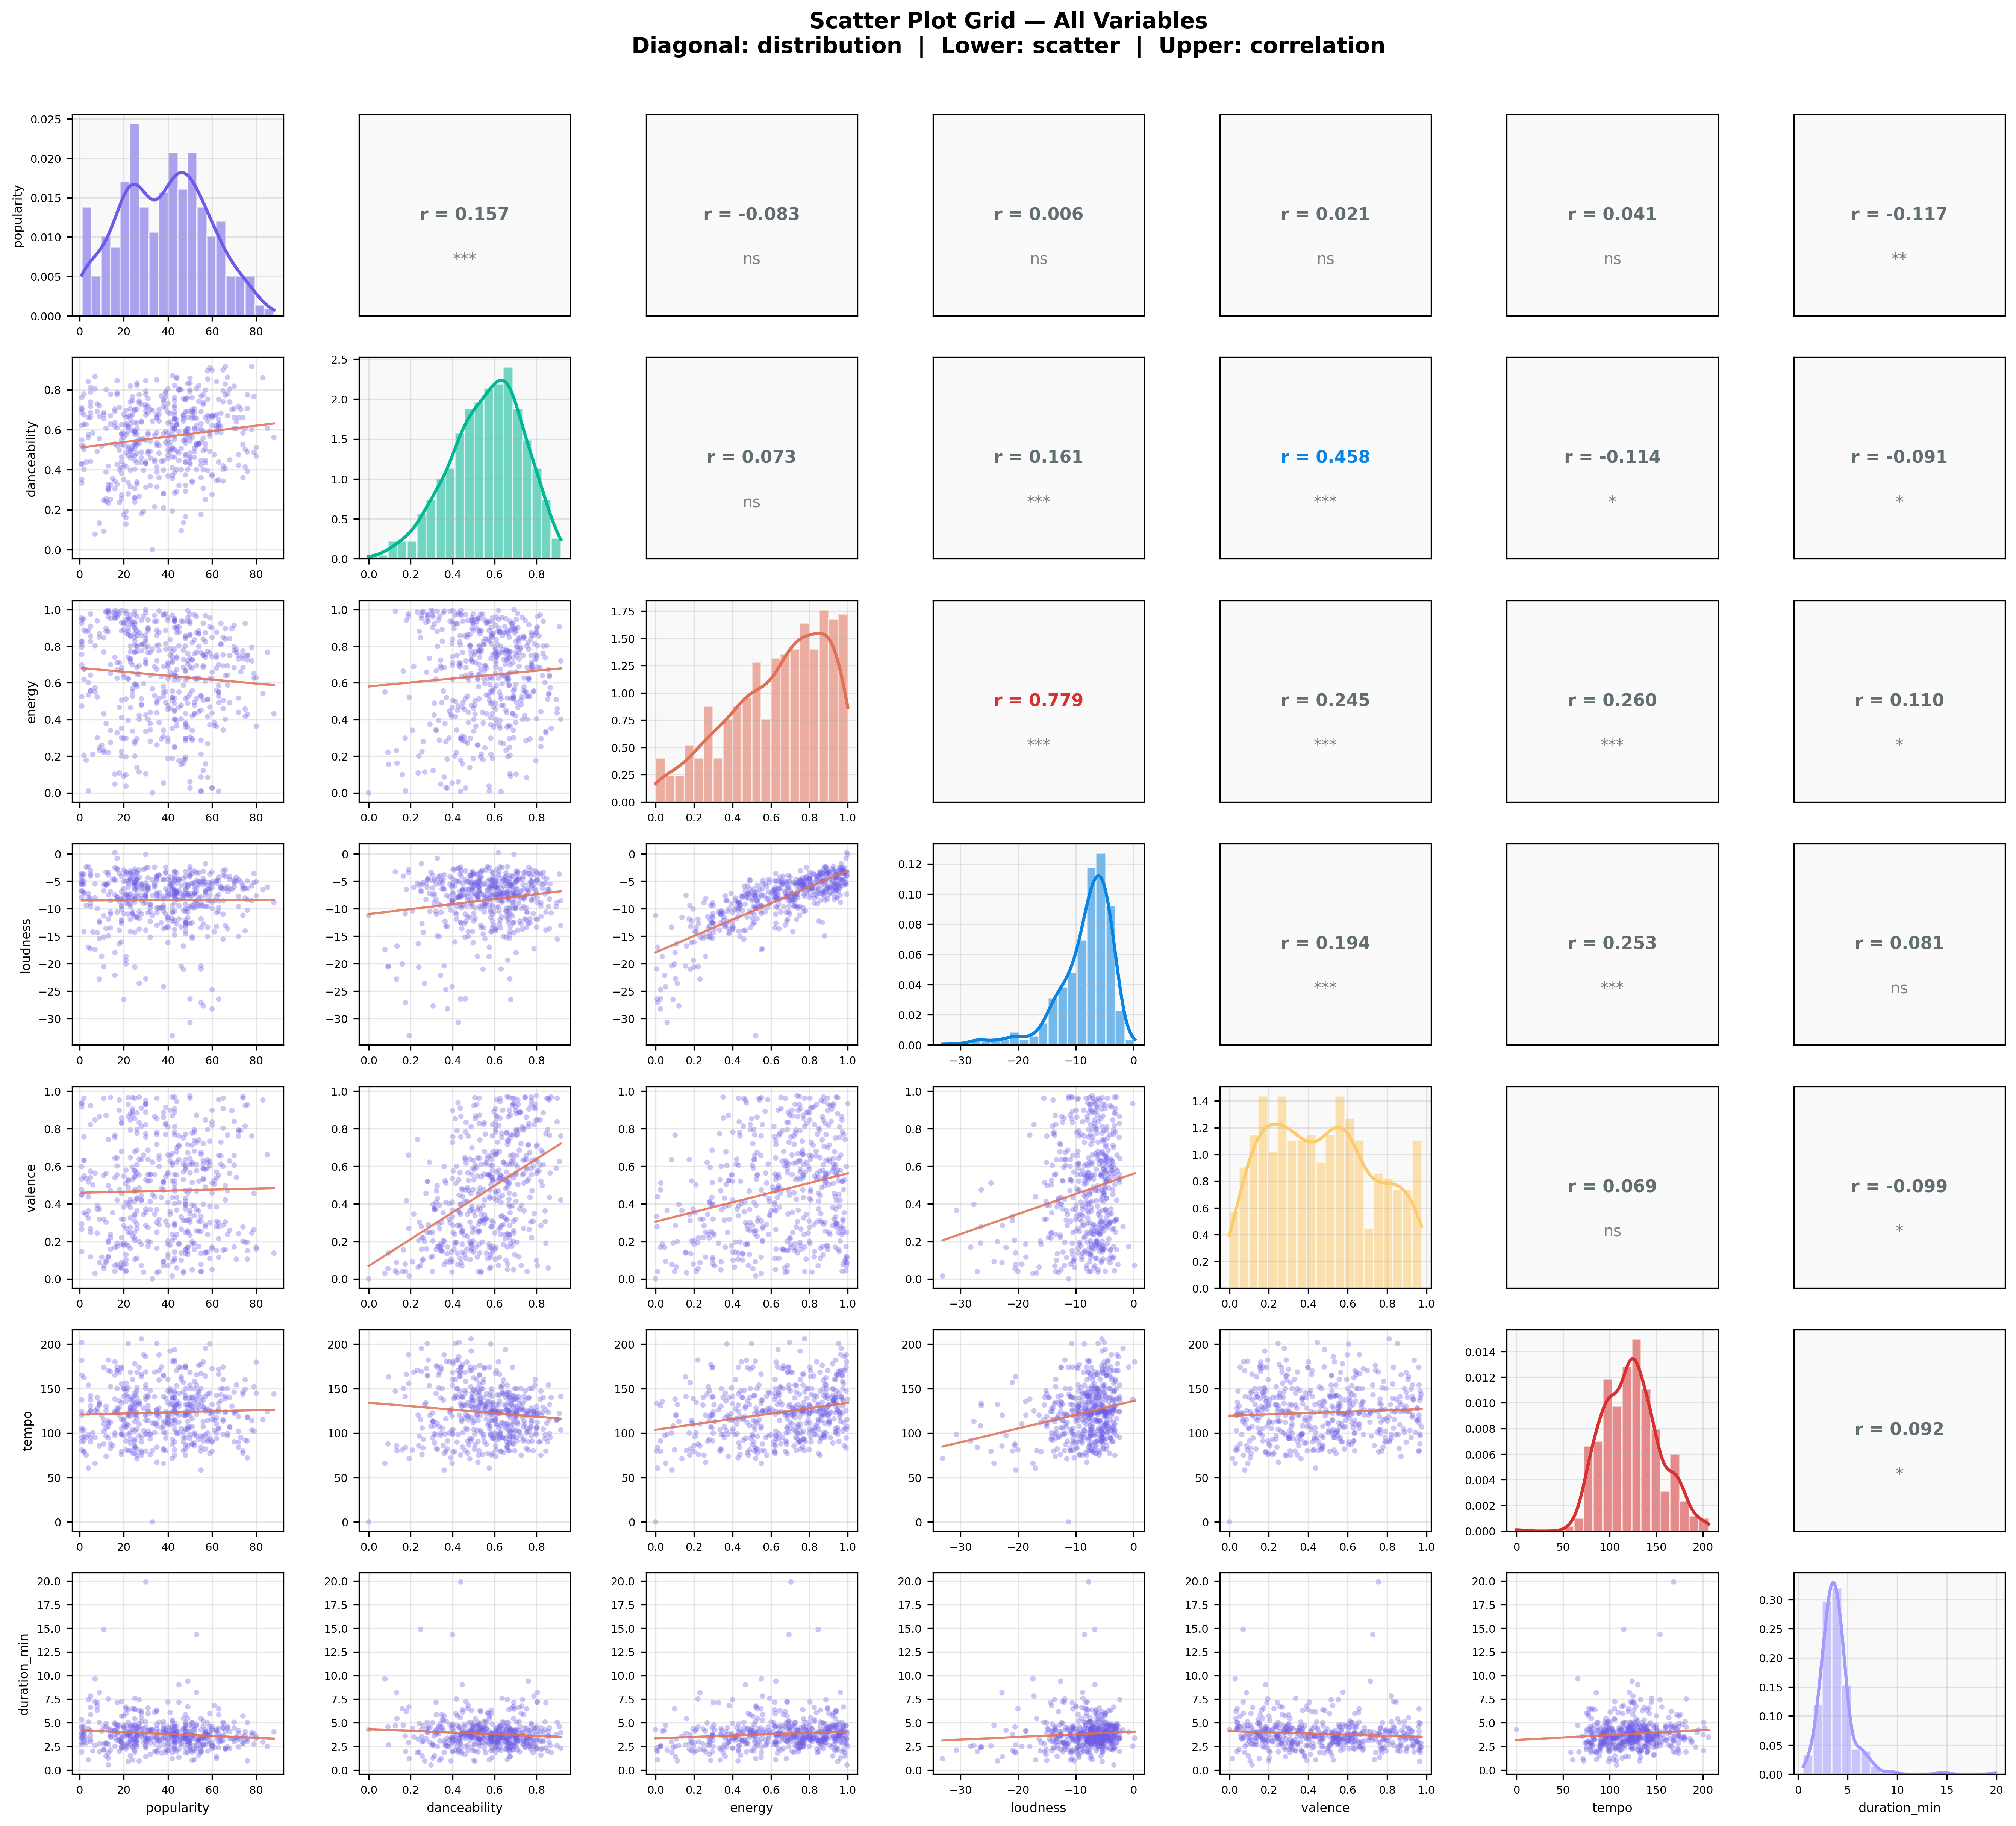
\includegraphics[width=\textwidth]{scatterplot_grid.png}
  \caption{Pairwise Scatter Grid. Lower: scatter + OLS line. Diagonal: KDE. Upper: Pearson $r$ with significance.}
\end{figure}

Key relationships: energy--loudness correlation is strongly positive (consistent with the physical link between signal power and perceived loudness). Popularity shows the strongest pairwise correlation with \texttt{tempo}.

%% 7. Model Estimation
\section{Estimation of Models}

\subsection{Multiple Linear Regression}
\begin{equation}
  \text{Popularity}_i = \beta_0 + \beta_1\,\text{Danceability}_i
  + \beta_2\,\text{Energy}_i + \beta_3\,\text{Loudness}_i
  + \beta_4\,\text{Valence}_i + \beta_5\,\text{Tempo}_i
  + \beta_6\,\text{Duration}_i + \varepsilon_i
\end{equation}

\textbf{Estimated equation:}
\begin{equation}
  \widehat{\text{Popularity}} = 35.6114 + 19.6636\,\text{danceability} - 10.2270\,\text{energy} + 0.2616\,\text{loudness} - 4.7140\,\text{valence} + 0.0715\,\text{tempo} - 1.4745\,\text{duration\ min}
\end{equation}

\begin{table}[H]
\centering\caption{OLS Estimation Results (Training, $n=400$)}
\begin{tabular}{lrrrrr}
\toprule
\textbf{Variable} & \textbf{Coef.} & \textbf{Std Err} & \textbf{t-stat} & \textbf{p-value} & \textbf{Sig.} \\
\midrule
  Intercept          &    35.6114 &     9.0833 &     3.9205 &     0.0001 &        \\
  danceability       &    19.6636 &     6.5281 &     3.0121 &     0.0028 &     ** \\
  energy             &   -10.2270 &     6.3962 &    -1.5989 &     0.1106 &     ns \\
  loudness           &     0.2616 &     0.3315 &     0.7890 &     0.4306 &     ns \\
  valence            &    -4.7140 &     4.2955 &    -1.0974 &     0.2731 &     ns \\
  tempo              &     0.0715 &     0.0344 &     2.0759 &     0.0386 &      * \\
  duration\_min      &    -1.4745 &     0.6858 &    -2.1501 &     0.0322 &      * \\
\midrule
\multicolumn{2}{l}{$R^2$} & \multicolumn{4}{l}{0.0486} \\
\multicolumn{2}{l}{Adj.\ $R^2$} & \multicolumn{4}{l}{0.0341} \\
\multicolumn{2}{l}{$F$-statistic} & \multicolumn{4}{l}{3.3492 ($p = 0.003134$)} \\
\multicolumn{2}{l}{AIC} & \multicolumn{4}{l}{3507.90} \\
\multicolumn{2}{l}{BIC} & \multicolumn{4}{l}{3535.84} \\
\bottomrule
\multicolumn{6}{l}{\small $^{*}p<0.05$, $^{**}p<0.01$, $^{***}p<0.001$, ns = not significant.}
\end{tabular}
\end{table}

\subsection{Random Forest Regressor}
$\hat{f}_{\text{RF}}(\mathbf{x}) = \frac{1}{B}\sum_{b=1}^{B} T_b(\mathbf{x})$, with $B = 500$ trees and \texttt{max\_features = 2}.

\begin{table}[H]
\centering\caption{RF Variable Importance (Mean Decrease in Impurity)}
\begin{tabular}{clr}
\toprule
\textbf{Rank} & \textbf{Variable} & \textbf{Importance} \\
\midrule
  1 & energy             & 0.202117 \\
  2 & loudness           & 0.178461 \\
  3 & duration\_min      & 0.159646 \\
  4 & valence            & 0.156190 \\
  5 & danceability       & 0.154179 \\
  6 & tempo              & 0.149407 \\
\bottomrule
\end{tabular}
\end{table}

%% 8. Results and Conclusion
\section{Results and Conclusion}

\subsection{Model Comparison}
\begin{figure}[H]
  \centering
  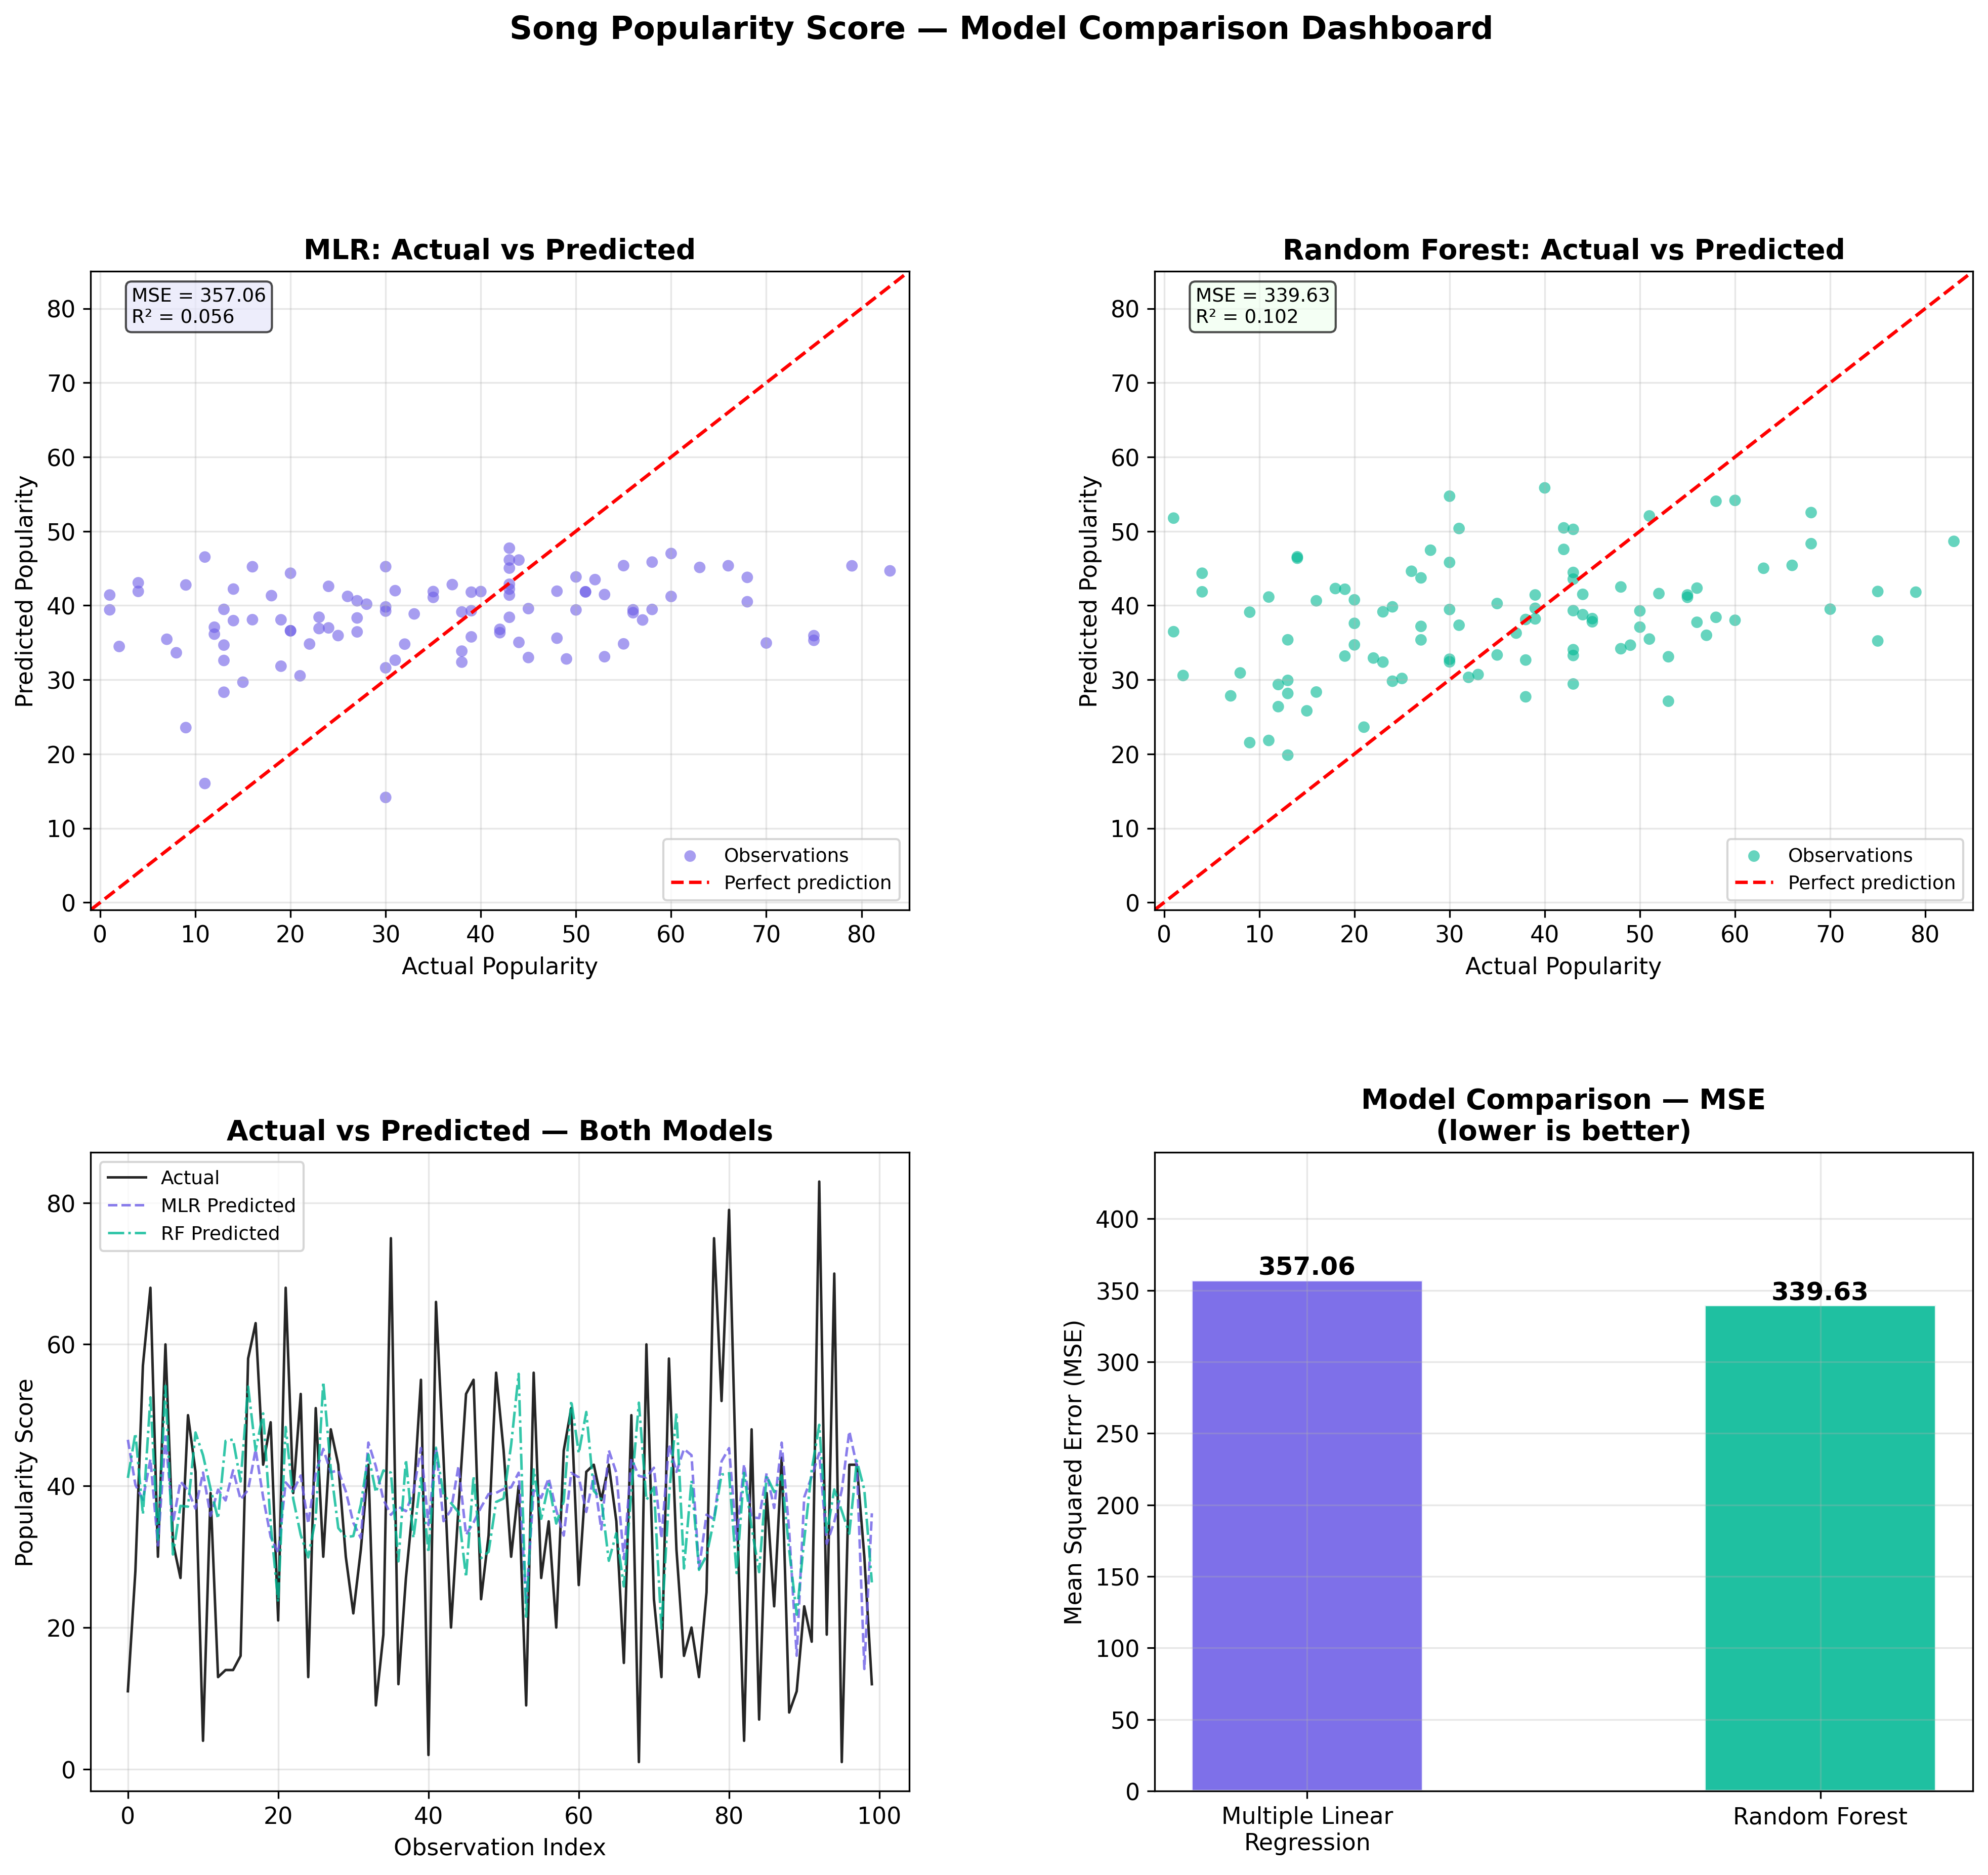
\includegraphics[width=\textwidth]{model_comparison.png}
  \caption{Model Comparison Dashboard.}
\end{figure}

\begin{figure}[H]
  \centering
  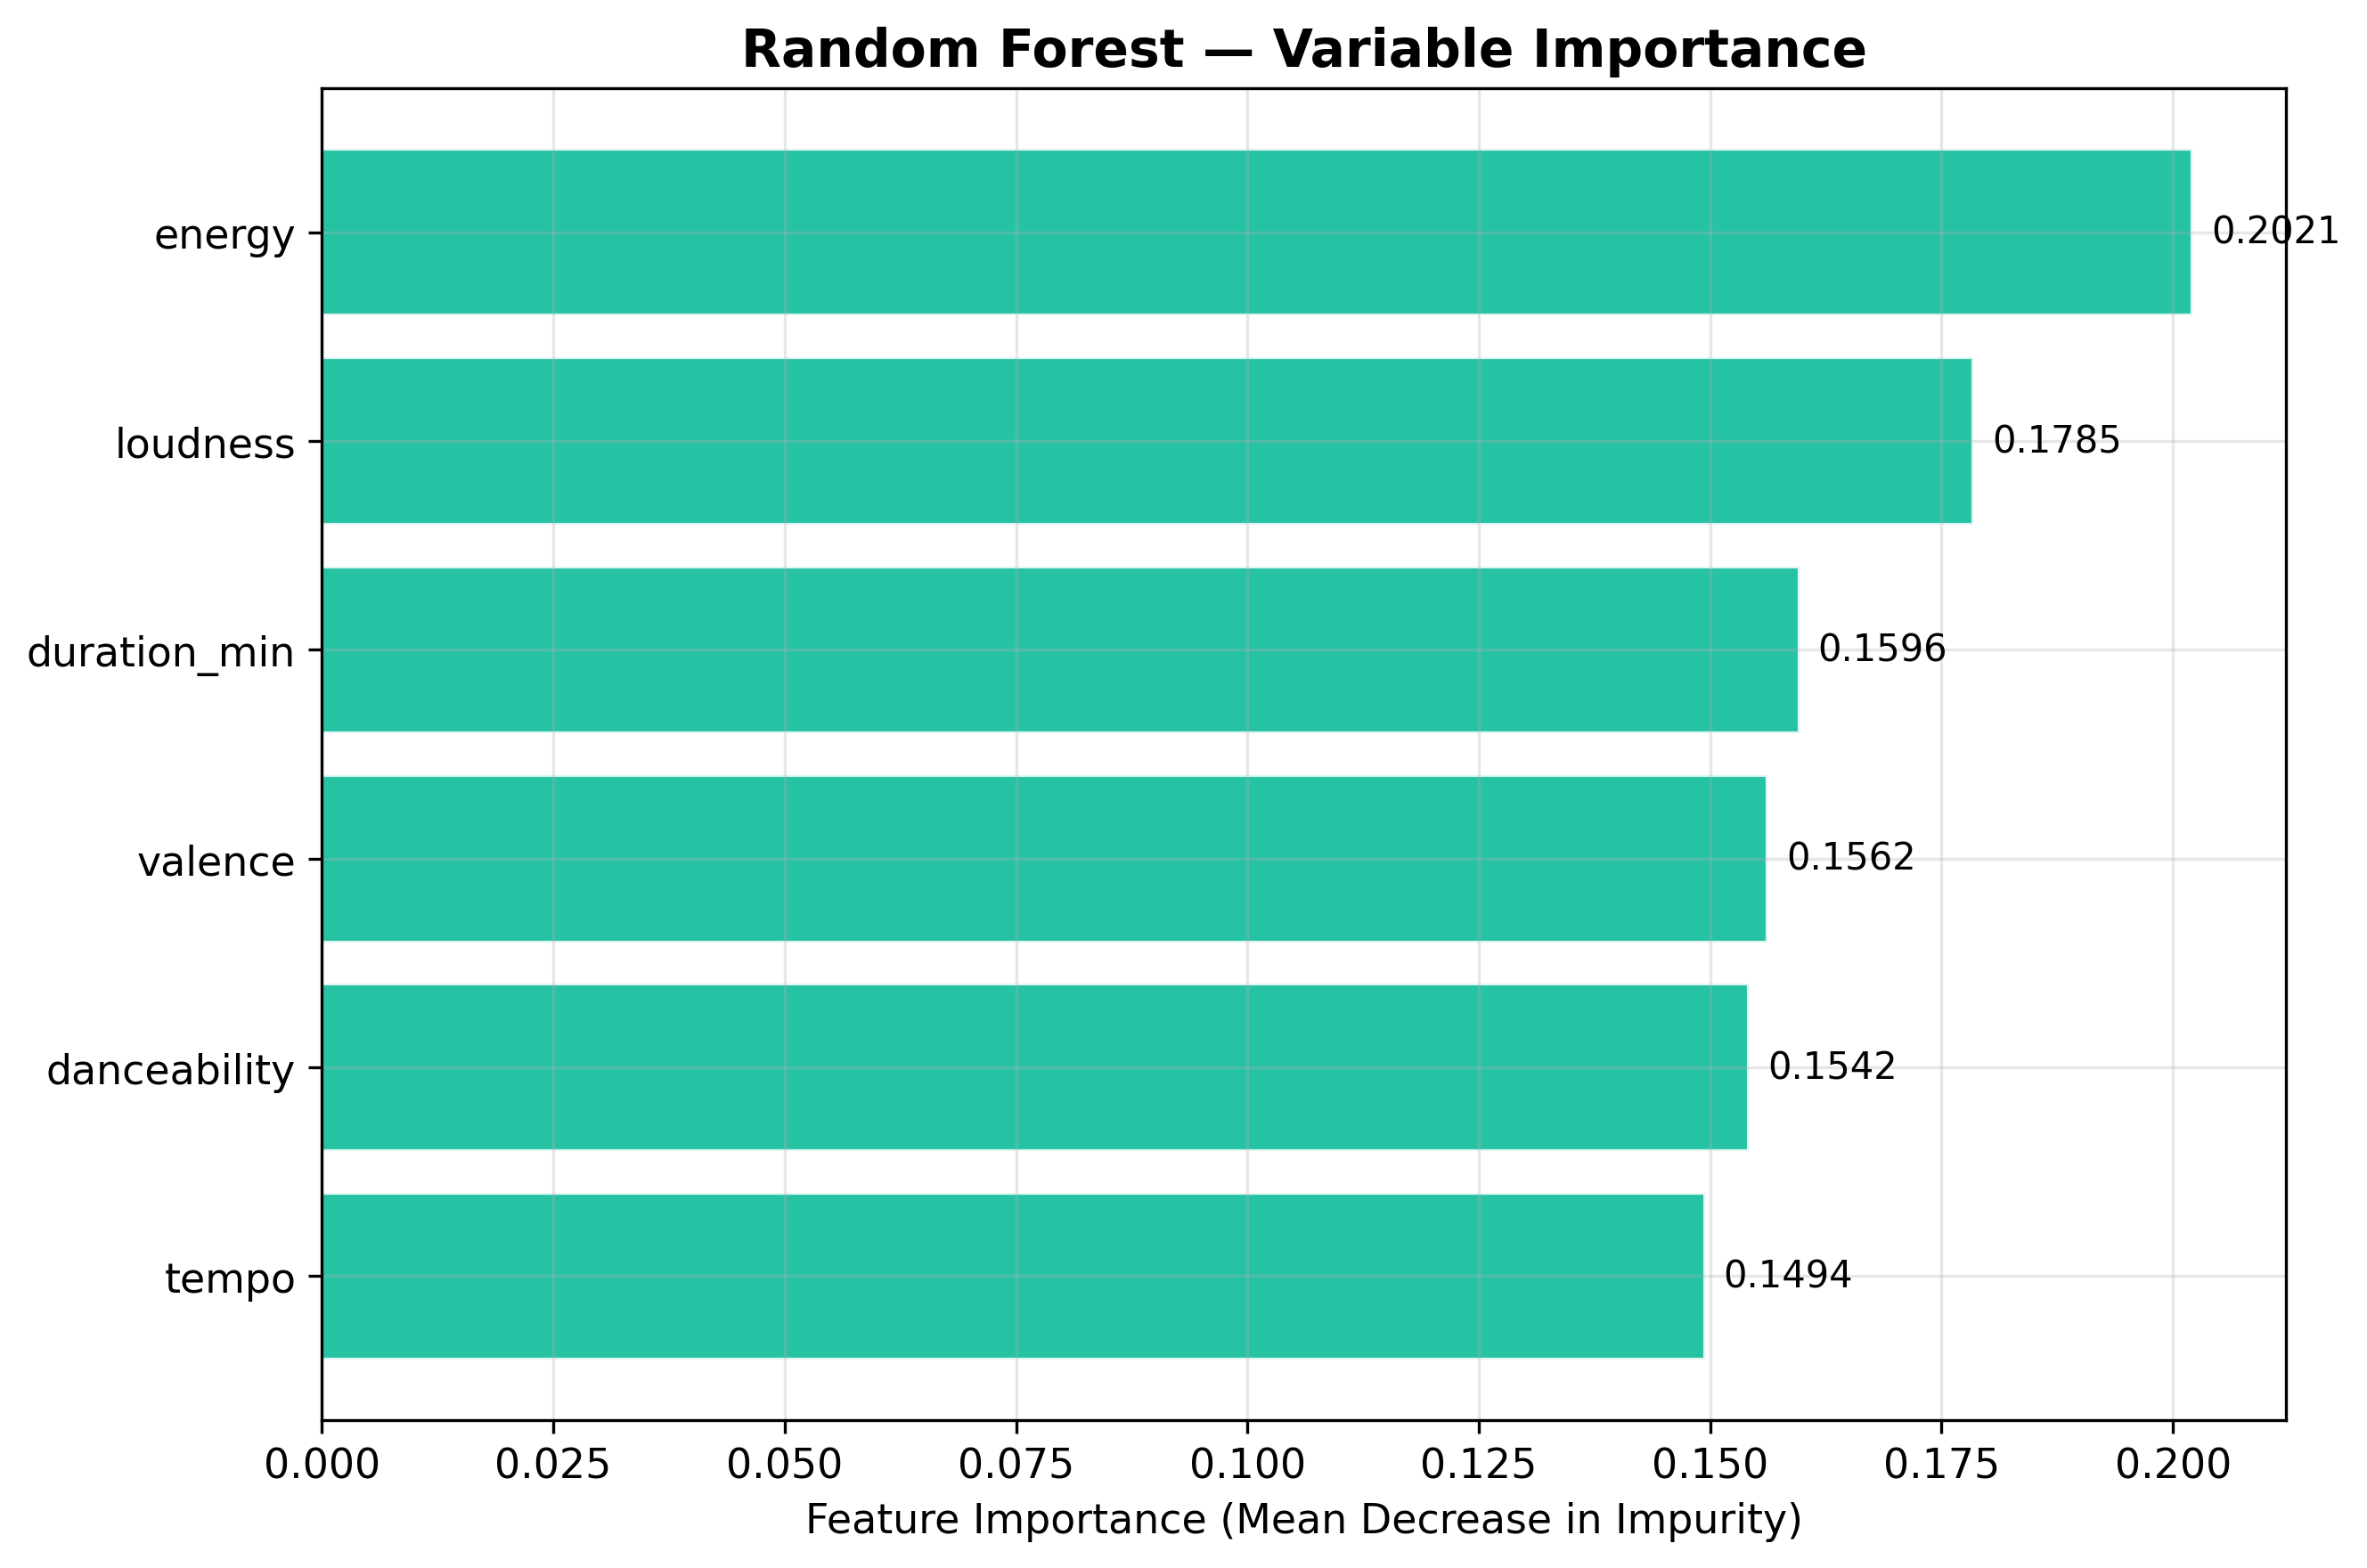
\includegraphics[width=0.8\textwidth]{variable_importance.png}
  \caption{Random Forest Variable Importance.}
\end{figure}

\begin{table}[H]
\centering\caption{Out-of-Sample Performance (Test Set, $n=100$)}
\begin{tabular}{lrrr}
\toprule
\textbf{Metric} & \textbf{MLR} & \textbf{Random Forest} & \textbf{Better} \\
\midrule
  MSE  & 357.0589 & 339.6295 & RF \\
  RMSE & 18.8960 & 18.4290 & RF \\
  MAE  & 15.4815 & 14.9935 & RF \\
  $R^2$ & 0.0555 & 0.1016 & RF \\
\bottomrule
\end{tabular}
\end{table}

\subsection{Conclusion}
This study examined six audio features as predictors of Spotify Popularity
Score using $n = 500$ tracks split into training (400) and test (100) sets.

The variables danceability, tempo, duration_min were statistically significant at the 5\% level ($p < 0.05$).
Loudness had a positive coefficient (0.2616), supporting H3. Duration had a negative coefficient (-1.4745), supporting H6. The model explains 4.9\% of the variance in popularity ($R^2 = 0.0486$).

The Random Forest achieved a lower test MSE (339.6295 vs 357.0589), confirming H7. The top predictors in the Random Forest were
\texttt{energy} and \texttt{loudness}, consistent with
Ferreri et al.\ (2019).

Both models underpredict extremely popular songs (scores $> 80$),
likely because viral hits involve social-media effects not captured
by audio features alone. Future work could add genre controls,
temporal trends, and playlist placement data.

%% References
\section*{References}
\addcontentsline{toc}{section}{References}
\bibliographystyle{apalike}
\bibliography{references}

\end{document}
